\section{OgreRenderer}
\label{chapter:implementation:ogrerenderer}

	The implementation of the \classname{Renderer} class using the Ogre3d library posed a few interesting problems.

	\subsection{Initialization}

		\subsubsection{Resource Locations}

			PURGE assumes that there is a pool of \classname{Model}s available for usage that can be addressed with a unique string identifier each. Fortunately, Ogre3d takes the same approach: During the initialization of the engine, one has to define a list of resource locations that contain such named objects. This means that the initialization of the \classname{OgreRenderer} itself must provide access to the functionality already present in Ogre3d.

			As this is the only parameter that needs to be specified at the start-up of the engine\footnote{All other parameters can operate with default values, but the location of the resources required by the application are taken to be of great interest to the developer using our API.}, we have decided to accept a resource location as a parameter to the factory.

			Ogre3d supports two different resource location classes containing resources -- both deriving from the \classname{Archive} interface: the \classname{FilesystemArchive} and the \classname{ZipArchive}, one providing access to files in a directory, the other granting access to files in zip-archive. As our library is aimed at rapid prototyping, we have chosen to support a single directory name as a resource location. Additional locations can be added using the API of Ogre3d itself, if required.

		\subsubsection{Delayed Initialization}

			Another issue arose during the implementation of the renderer on Linux. The application was crashing if an Ogre::Camera was created an Ogre::Window. A similar crash occurred when the resource locations were registered before a Window was established. Both issues turned out to be a constraint imposed by OpenGL: Several operations in OpenGL require a window as a context.
			
			The solution was to delay the initialization of the complete \classname{OgreRenderer} until a \classname{PURGE::Window} was defined. This approach has no side effects, as the rendered output on the window is the single duty of the \classname{Renderer}. The method \inlinecode{perform()} would return immediately without performing any operations either way.
			
	\subsection{Communication}

		The communication between the two libraries is handled at a central point, the \classname{Transcription} class, outlined in Figure \ref{fig:Transcription}. This template class uses the curiously recurring template pattern -- just like its management counterpart in PURGE, the \classname{TrackedObject}, outlined in Figure \ref{fig:TrackedObject} -- and provides two static functions for synchronizing PURGE objects and their corresponding bridge objects:

		\begin{figure}[htbp]
			\centering
			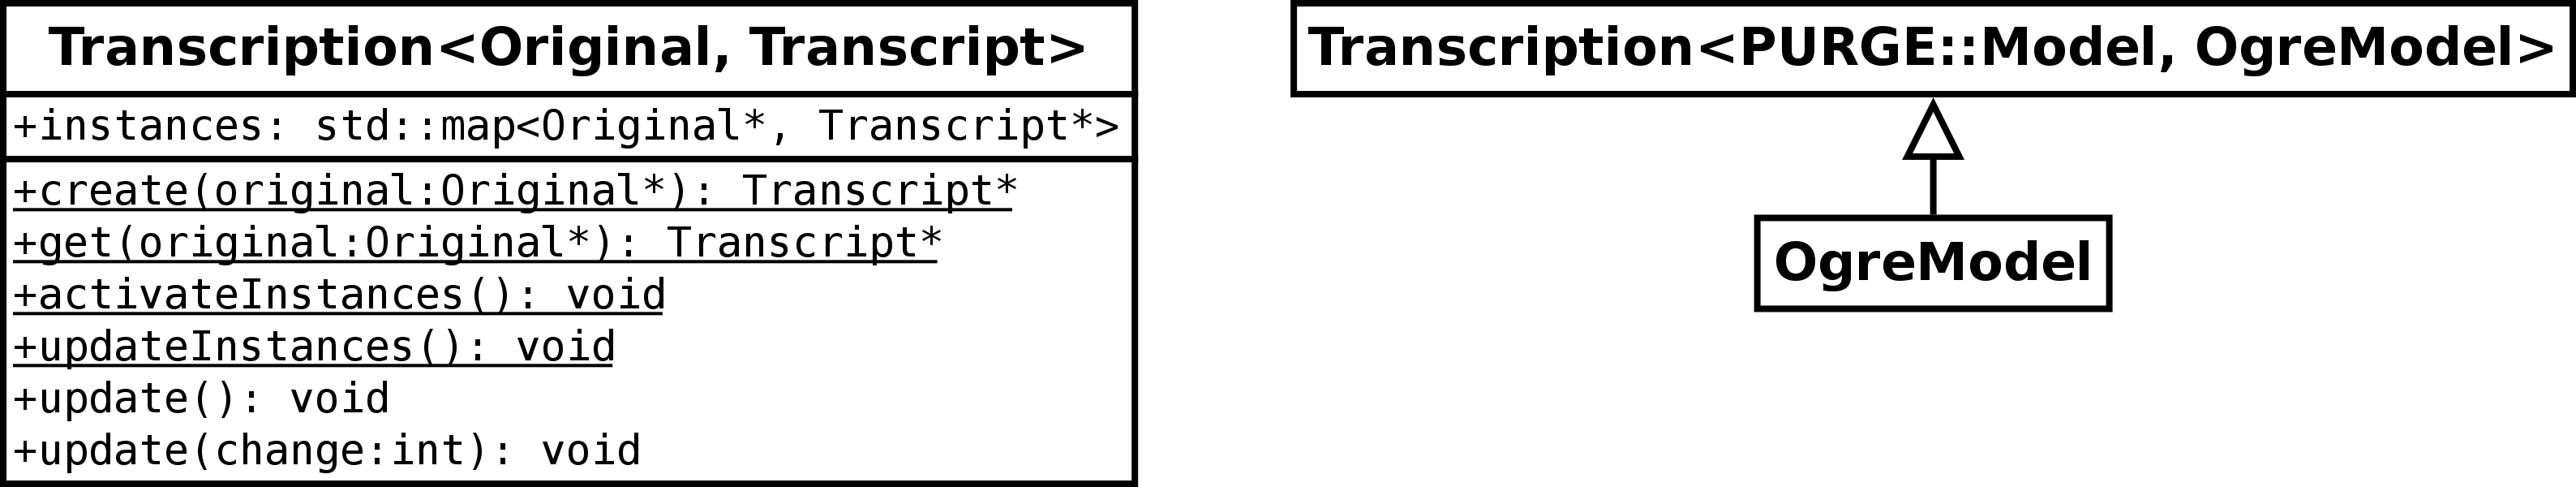
\includegraphics[width=14cm]{images/Transcription.png}
			\caption{The \classname{Transcription} class manages the communication between PURGE objects and Ogre3d objects.}
			\label{fig:Transcription}
		\end{figure}

		\begin{smalllist}
			\item \inlinecode{activateInstances()} will read all available objects in PURGE and create matching instances in the \classname{OgreRenderer}. This step is only necessary to activate the renderer.
			\item \inlinecode{updateInstances()} is called by \inlinecode{OgreRenderer::render()} prior to the rendering. It creates new objects, destroys obsolete objects and carries any modified state from the existing PURGE objects to the bridge objects.
		\end{smalllist}

		Both procedures possibly create bridge objects. To provide greater flexibility for this purpose, the classes assume a static factory method instead of calling the constructor directly. The \classname{Transcript} template parameter has the option of implementing this factory to perform additional operations after the object was created.

